\chapter{Matheuristics}
Matheuristics, a fusion of mathematical programming and metaheuristic techniques, have emerged as robust and versatile approaches for solving complex optimization problems.
These hybrid methods leverage the strengths of both mathematical programming, which provides exact and rigorous solutions, and metaheuristics, which offer flexibility and the ability to escape local optima.
By integrating these two paradigms, matheuristics aim to efficiently solve large-scale and complex problems that are otherwise intractable using conventional methods alone.
This chapter will address two Matheuristics, \textbf{Hard Fixing} and \textbf{Local Branching}, which rely on the use of CPLEX to optimize an already existing solution.

\section{Hard Fixing}
Hard Fixing is a Matheuristic that optimize an already feasible TSP solution "fixing" in place some of the edges of the solution and the optimizing the rest using CPLEX.
This approach begins with the generation of an initial feasible solution, typically derived from a heuristic or metaheuristic method such as Tabu Search or Variable Neighborhood Search.
Once an initial solution is obtained, the process of "hard fixing" commences.
In this context, hard fixing refers to selecting a subset of the solution's components and fixing them in place.
This reduces the problem size and complexity for subsequent optimization steps.
There are multiple ways to choose which edges to fix and which edges to keep "free":

\begin{itemize}
    \item \textbf{Random Fix}\\
    The easiest method to implement is to fix edges in the solution at random up to a certain threshold.
    As far as effectivenss goes, this method relies mostly on luck since it's a completely random method the change of locking a set of edges that allows a good optimization can be selected purely by chance.
    \begin{figure}[H]
        \centering
        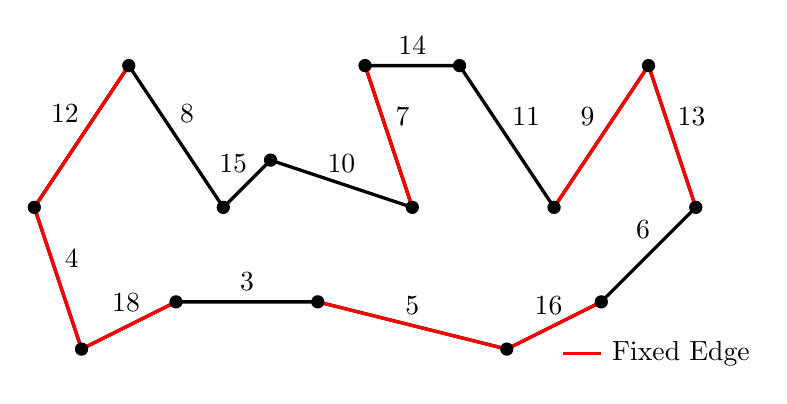
\begin{tikzpicture}[thick,scale=.6]
            \coordinate (A) at (0, 0);\coordinate (B) at (2, 3);\coordinate (C) at (4, 0);\coordinate (D) at (1, -3);\coordinate (E) at (3, -2);\coordinate (F) at (5, 1);\coordinate (G) at (6, -2);\coordinate (H) at (8, 0);\coordinate (I) at (7, 3);\coordinate (J) at (9, 3);\coordinate (K) at (11, 0);\coordinate (L) at (10, -3);\coordinate (M) at (12, -2);\coordinate (N) at (14, 0);\coordinate (O) at (13, 3);

            \draw[-,very thick] (A) -- node[above,yshift=1,xshift=-6] {12} (B) -- node[above,yshift=1,xshift=4] {8} (C) --node[above,xshift=-5] {15} (F) -- node[above] {10} (H) -- node[above,xshift=5] {7} (I) -- node[above] {14} (J) -- node[above,xshift=7] {11} (K) -- node[above,xshift=-5] {9} (O) -- node[above,xshift=7] {13} (N) -- node[above,yshift=2,xshift=-2] {6} (M) -- node[above,xshift=-2] {16} (L) -- node[above] {5} (G) -- node[above] {3} (E) -- node[above,yshift=1,xshift=-1] {18} (D) -- node[above,xshift=5] {4} (A);
            \draw[-,very thick, Red] (A) -- (B);
            \draw[-,very thick, Red] (H) -- (I);
            \draw[-,very thick, Red] (K) -- (O);
            \draw[-,very thick, Red] (O) -- (N);
            \draw[-,very thick, Red] (E) -- (D);
            \draw[-,very thick, Red] (M) -- (L);
            \draw[-,very thick, Red] (L) -- (G);
            \draw[-,very thick, Red] (D) -- (A);

            \foreach \point in {A, B, C, D, E, F, G, H, I, J, K, L, M, N, O} {
                \fill (\point) circle (4pt);
            }

            \draw [-,very thick,Red] (11.2,-3.1) --  (12,-3.1) node[anchor=west, black] {Fixed Edge};
        
        \end{tikzpicture}
	    \caption{Example of a random fix of 8 edges} \label{fig:exampleRndFix}
    \end{figure}
    \item \textbf{Smallest Edges Fix}\\
    To fix edges based on their cost is a greedy technique that consists in fixing the first $n$ edges sorted in ascending order by cost.
    This makes that only the edges in the solution with the greatest cost are allowed to be removed from the solution.
    The avantage here is that intuitevly speaking the most expensive nodes in the solution are the ones that can usually be swapped with some move with cheaper edges.
    The downside is that, once the optimal solution is found among the most expensive edges in the solution, the optimization gets stuck in a local minimum.
    \begin{figure}[H]
        \centering
        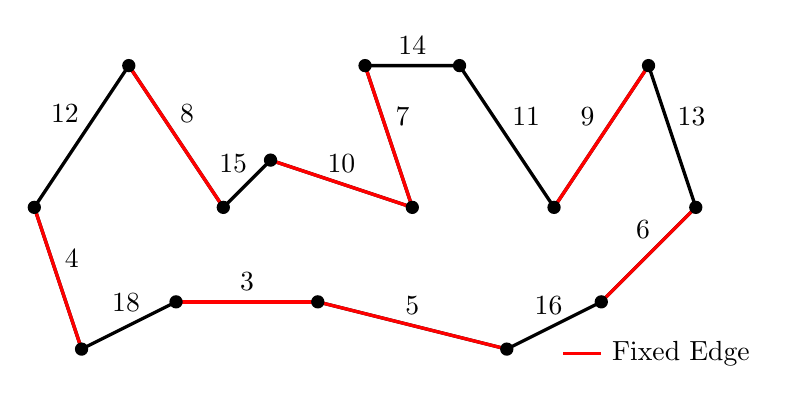
\begin{tikzpicture}[thick,scale=.6]
            \coordinate (A) at (0, 0);\coordinate (B) at (2, 3);\coordinate (C) at (4, 0);\coordinate (D) at (1, -3);\coordinate (E) at (3, -2);\coordinate (F) at (5, 1);\coordinate (G) at (6, -2);\coordinate (H) at (8, 0);\coordinate (I) at (7, 3);\coordinate (J) at (9, 3);\coordinate (K) at (11, 0);\coordinate (L) at (10, -3);\coordinate (M) at (12, -2);\coordinate (N) at (14, 0);\coordinate (O) at (13, 3);

            \draw[-,very thick] (A) -- node[above,yshift=1,xshift=-6] {12} (B) -- node[above,yshift=1,xshift=4] {8} (C) --node[above,xshift=-5] {15} (F) -- node[above] {10} (H) -- node[above,xshift=5] {7} (I) -- node[above] {14} (J) -- node[above,xshift=7] {11} (K) -- node[above,xshift=-5] {9} (O) -- node[above,xshift=7] {13} (N) -- node[above,yshift=2,xshift=-2] {6} (M) -- node[above,xshift=-2] {16} (L) -- node[above] {5} (G) -- node[above] {3} (E) -- node[above,yshift=1,xshift=-1] {18} (D) -- node[above,xshift=5] {4} (A);
            \draw[-,very thick, Red] (G) -- (E);
            \draw[-,very thick, Red] (D) -- (A);
            \draw[-,very thick, Red] (L) -- (G);
            \draw[-,very thick, Red] (N) -- (M);
            \draw[-,very thick, Red] (B) -- (C);
            \draw[-,very thick, Red] (H) -- (I);
            \draw[-,very thick, Red] (K) -- (O);
            \draw[-,very thick, Red] (F) -- (H);

            \foreach \point in {A, B, C, D, E, F, G, H, I, J, K, L, M, N, O} {
                \fill (\point) circle (4pt);
            }

            \draw [-,very thick,Red] (11.2,-3.1) --  (12,-3.1) node[anchor=west, black] {Fixed Edge};
        \end{tikzpicture}
	    \caption{Example of a smallest edges fix of 8 edges} \label{fig:exampleSmallFix}
    \end{figure}
    \item \textbf{Sequence Fix}\\
    Fixing along a sequence means that edges are locked starting from a node, following the path of the known solution until the desired number of nodes have been locked.
    On the upside this technique allows to optimize contigous sections of the solution, resulting in obtaining piecese of solution that, taken alone, have reached optimality.
    The disadvantage is that this method allows only localized moves, while completely negleting optimizations that view the problem with a wider angle.
    \begin{figure}[H]
        \centering
        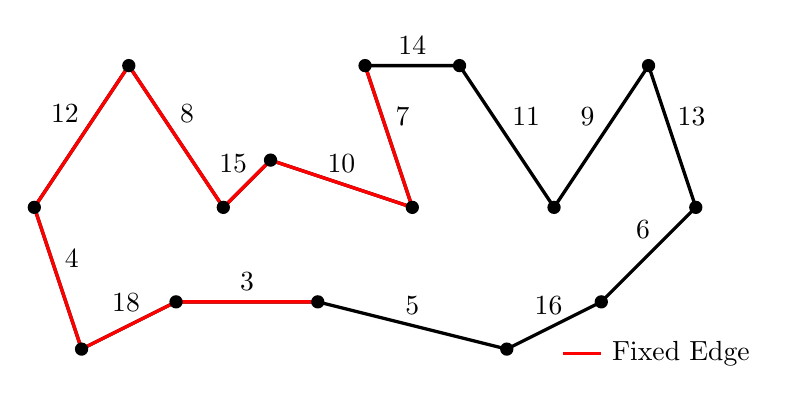
\begin{tikzpicture}[thick,scale=.6]
            \coordinate (A) at (0, 0);\coordinate (B) at (2, 3);\coordinate (C) at (4, 0);\coordinate (D) at (1, -3);\coordinate (E) at (3, -2);\coordinate (F) at (5, 1);\coordinate (G) at (6, -2);\coordinate (H) at (8, 0);\coordinate (I) at (7, 3);\coordinate (J) at (9, 3);\coordinate (K) at (11, 0);\coordinate (L) at (10, -3);\coordinate (M) at (12, -2);\coordinate (N) at (14, 0);\coordinate (O) at (13, 3);

            \draw[-,very thick] (A) -- node[above,yshift=1,xshift=-6] {12} (B) -- node[above,yshift=1,xshift=4] {8} (C) --node[above,xshift=-5] {15} (F) -- node[above] {10} (H) -- node[above,xshift=5] {7} (I) -- node[above] {14} (J) -- node[above,xshift=7] {11} (K) -- node[above,xshift=-5] {9} (O) -- node[above,xshift=7] {13} (N) -- node[above,yshift=2,xshift=-2] {6} (M) -- node[above,xshift=-2] {16} (L) -- node[above] {5} (G) -- node[above] {3} (E) -- node[above,yshift=1,xshift=-1] {18} (D) -- node[above,xshift=5] {4} (A);
            \draw[-,very thick, Red] (G) -- (E) -- (D) -- (A) -- (B) -- (C) -- (F) -- (H) -- (I);

            \foreach \point in {A, B, C, D, E, F, G, H, I, J, K, L, M, N, O} {
                \fill (\point) circle (4pt);
            }

            \draw [-,very thick,Red] (11.2,-3.1) --  (12,-3.1) node[anchor=west, black] {Fixed Edge};
        \end{tikzpicture}
	    \caption{Example of a sequence fix of 8 edges} \label{fig:exampleSeqFix}
    \end{figure}
\end{itemize}
Since every one of these techniques have different advantages and disadvantages, a good strategy is to choose at random which method to use to fix edges at every iteration.
Even by using all of these procedure together there is the risk of becoming stuck in a local minima.
There surely exist a lot of ways to escape a local minimum point, the simplest one is just to reduce the amount of fixed edges once the solution stops improving.
To roughly detect the local minima one can simply check how many iterations from the last improving iteration have been performed.
Then, after a threshold value of not-improving iterations has been crossed just decrease the number of fixed edges.
In this implementation, the starting number of fixed edges is 10\% the number of nodes and it is decreased with steps of equal size.
\begin{figure}[htbp]
	\begin{algorithm}[H]
        \TitleOfAlgo{\textbf{Hard Fixing}}
		\SetKwInOut{Input}{input}
        \SetKwInOut{Output}{Output}
		\Input{
			Starting solution $s$ \newline
            Time limit $tlim$ \newline
            Number of edges to fix $n$ \newline
            Stagnant iterations threshold $iterThresh$
		}
        \Output{Improved solution $s$}
		\vspace{2mm}
        $p \gets$ CPLEX Initialization \\
        $i \gets 0$ \\ 
        \While{$time < tlim$}{
            fix $n$  edges in $p$ according to one of the 3 methods chosen at random\\
            run Branch and Cut on $p$ \\
            $x^* \gets$ optimal solution of $p$ (w.r.t. the fixed edges) \\
            $s' \gets$ convert $x^*$ to successors solution \\
            \eIf{$cost(s') < cost(s)$}{
                $s \gets s'$\\
                $i \gets 0$
            }{
                $i++$\\
                \lIf{$i = iterThresh$}{
                    \textbf{decrease} $n$
                }
            }
            \uIf{$n$ = 0}{
                \textbf{break}
                \tcp{Optimal solution found}
            }
            un-fix all previously fixed edges in $p$
        }
        \textbf{return} $s$
	\end{algorithm}
	\caption{Pseudocode of the Hard Fixing algorithm} \label{fig:hardfix}
\end{figure}

\subsection{Performance}

Even though matheuristics are written on top of the exact method Branch and Cut, their output solution is not guaranteed to be optimal since, from a high level viewpoint, their behavior is more comparable to a metaheuristic.
Therefore it makes sense for algorithms like Hard Fixing to be analyzed on the quality of the output solution.
\figurename{ \ref{fig:hardfixCost}} does exactly that, showing the difference between the cost of the solution used as input, the output solution as well as the optimal solution, in order to derive meaningful conclusion on the performance of the algorithm.
\begin{figure}[htbp]
	\centering
    \begin{tikzpicture}
        \begin{axis}[
            xlabel={Cost Ratio},     % AXIS NAME
            %ylabel={Iterations/s Ratio},   % AXIS NAME
            xmin=1, xmax=1.1,       % AXIS LIMITS
            ymin=0, ymax=67,        % AXIS LIMITS
            xtick={},
            ytick=\empty,
            legend style={at={(0.98,0.02)},anchor=south east,legend columns=1}, %MOVE LEGEND HERE
			legend cell align={left},
            %ymajorgrids=true,
            xmajorgrids=true,
            grid style=dashed,
        ]
        
        \addplot[Blue,mark=square,mark size=1.5] table[x=startcost,y=idx, col sep=semicolon] {csv/hardfix_cost.csv}; 
        \addplot[Red,mark=o,mark size=1.5] table[x=finalcost,y=idx, col sep=semicolon] {csv/hardfix_cost.csv};
        \addplot[Green,mark=triangle,mark size=1.5] table[x=optimalcost,y=idx, col sep=semicolon] {csv/hardfix_cost.csv}; 
        \addlegendentry{Starting Cost} 
        \addlegendentry{Final Cost}
        \addlegendentry{Optimal Cost}
            
        \end{axis}
    \end{tikzpicture}
	\caption{Performance profile graph of Hard Fixing\label{fig:hardfixCost}}
\end{figure}
Like with the other algorithms using CPLEX shown before, the time limit set to find the initial solution was set to 1\% of the full time limit.
The initial solution was obtained using Nearest Neighbor and 2-Opt.
% Time limits are set as follows:
% \begin{itemize}
%     \item from 0 to 80 nodes, 1 second
%     \item form 100 to 200 nodes, 3 seconds
%     \item from 220 to 320 nodes, 8 seconds
%     \item from 400 to 500 nodes, 20 seconds
%     \item from 500 to 800 nodes, 60 seconds
%     \item from 1000 to 1440 nodes, 180 seconds
%     \item from 1440 to 2400 nodes, 400 seconds
% \end{itemize}
\begin{table}[htbp]
	\centering
	\begin{tabular}{c|c|c|}
        & \textbf{Optimization Amount} & \textbf{Distance from Optimal} \\
		\hline \textbf{mean} & 3.34\% & 0.96\% \\
		\hline \textbf{std dev} & 1.70\% & 1.08\% \\
        \hline \textbf{Q(25\%)} & 2.23\% & 0.14\% \\
        \hline \textbf{Q(50\%)} & 3.39\% & 0.47\% \\
        \hline \textbf{Q(75\%)} & 4.25\% & 1.42\% \\
	\end{tabular}
    \vspace{2mm}
	\caption{Statistics on results from Hard Fixing} \label{tab:hardfixStats}
\end{table}

\section{Local Branching}

Local Branching is a matheuristic technique that basically performes a series of "k-Opt" move to improve the solution.
Like Hard Fixing, it begins with a feasible initial solution, which can be generated using various heuristics or metaheuristics.
This initial solution serves as a starting point for the local branching process.
In Local Branching, a neighborhood of the current solution is defined by introducing additional constraints, known as local branching constraints.
These constraints limit the search to a subset of solutions that are "close" to the current solution in terms of some predefined criteria, such as the number of differing edges in the TSP tour.
By restricting the search to this localized region, the optimization process can focus on improving the solution within a manageable computational effort.
The optimization within this local neighborhood is performed using mathematical programming techniques, in this case, the Branch and Cut algorithm implemented with CPLEX is used.
The solver explores this restricted solution space to find an improved solution.
If an improved solution is found, it becomes the new incumbent solution, and a new neighborhood is defined around it.
This iterative process of defining local neighborhoods and optimizing within them continues until a stopping criterion is met, in this case a time limit.

\begin{figure}[htbp]
    \centering
    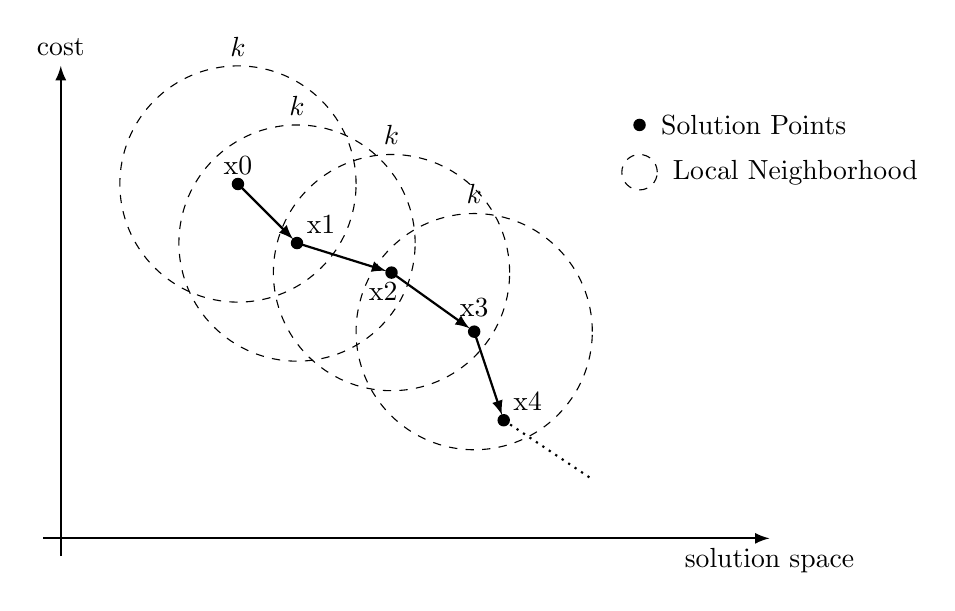
\begin{tikzpicture}[scale=.75]

        \draw[-latex,thick] (-6,-2.3) -- (-6,6) node[above]{cost};
        \draw[-latex,thick] (-6.3,-2) -- (6,-2) node[below]{solution space};

        % Define coordinates for initial, intermediate, and final solutions
        \coordinate (init) at (-3, 4);
        \coordinate (int1) at (-2, 3);
        \coordinate (int2) at (-0.4, 2.5);
        \coordinate (int3) at (1, 1.5);
        \coordinate (final) at (1.5, 0);
        \coordinate (beyond) at (3,-1);
        
        % Draw the initial, intermediate, and final solutions as points
        \fill (init) circle (3pt) node[above] {x0};
        \fill (int1) circle (3pt) node[above right] {x1};
        \fill (int2) circle (3pt) node[below, xshift=-3] {x2};
        \fill (int3) circle (3pt) node[above, yshift=2] {x3};
        \fill (final) circle (3pt) node[above right] {x4};
        
        % Draw arrows to show the progression
        \draw[-latex,thick,shorten <=2pt,shorten >=2pt] (init) -- (int1);
        \draw[-latex,thick,shorten <=2pt,shorten >=2pt] (int1) -- (int2);
        \draw[-latex,thick,shorten <=2pt,shorten >=2pt] (int2) -- (int3);
        \draw[-latex,thick,shorten <=2pt,shorten >=2pt] (int3) -- (final);
        \draw[thick,dotted] (final) -- (beyond);
        
        % Draw a few example neighborhoods
        \draw[dashed] (init) circle (2) + (0,2) node[above]{$k$};
        \draw[dashed] (int1) circle (2) + (0,2) node[above]{$k$};
        \draw[dashed] (int2) circle (2) + (0,2) node[above]{$k$};
        \draw[dashed] (int3) circle (2) + (0,2) node[above]{$k$};
        
        % Add a legend
        \fill (3.8, 5) circle (3pt);
        \node[right] at (4, 5) {Solution Points};
        \draw[dashed] (3.8, 4.2) circle (0.3);
        \node[right] at (4.2, 4.2) {Local Neighborhood};
        
    \end{tikzpicture}
	\caption{Example of Local Branching optimizing iterations } \label{fig:locBrancSolDescent}
\end{figure}    

The implementation of this matheuristic is not much different from the implementation of Hard Fixing.
Of course the initial solution will be used to initialize the CPLEX problem and the Branch and Cut algorithm will be used as well.
The differences with Hard Fixing is in the way the CPLEX problem is modified: instead of changing the lower bound of variables a new constraint is added.
Given $n$ as the number of nodes, $S = \{(a,b),(b,c),(c,d),...\}$ as the starting solution, $|S| = n$, and $k$ as the neighborhood size, the \textbf{locality constraint} is defined as follows
\[
    \sum_{e \in S} x_e >= n-k
\]
Of course, as it was the case with all 2-Opt, there is the risk in becoming stuck into a local minima solution for a given value of $k$.
When that happens, metaheuristics like Variable Neighborhood Search and Tabu Search used the techniques of performing some kind of non-improving moves so to escape the local minimum point.
In Local Branching it's not necessary to use such a technique since it's possible to increase $k$ without any efforts, allowing to escape the local minima at the cost of a harder problem for Branch and Cut to solve.
After the algorithm escapes the critical point it's possible to reduce again the value of $k$, to return to the original problem complexity.
In this implementation $k$ starts out with the value of 10 and it is increased, when necessary, by 5.

\begin{figure}[htbp]
	\begin{algorithm}[H]
        \TitleOfAlgo{\textbf{Local Branching}}
		\SetKwInOut{Input}{input}
        \SetKwInOut{Output}{Output}
		\Input{
			Starting solution $s$ \newline
            Time limit $tlim$ \newline
            Neighborhood size $k$
		}
        \Output{Improved solution $s$}
		\vspace{2mm}
        $p \gets$ CPLEX Initialization \\
        $i \gets 0$ \\ 
        \While{$time < tlim$}{
            add locality constraint to $p$\\
            run Branch and Cut on $p$ \\
            $x^* \gets$ optimal solution of $p$ (w.r.t. the restricted solution space) \\
            $s' \gets$ convert $x^*$ to successors solution \\
            \eIf{$cost(s') < cost(s)$}{
                $s \gets s'$
            }{
                \textbf{increase} $k$\\
            }
            \uIf{$k$ = number of nodes}{
                \textbf{break}
                \tcp{Optimal solution found}
            }
            remove locality constraint from $p$
        }
        \textbf{return} $s$
	\end{algorithm}
	\caption{Pseudocode of the Local Branching algorithm} \label{fig:localBranching}
\end{figure}

\subsection{Performance}

The data shown by \figurename{ \ref{fig:localBranchingCost}} and \tablename{ \ref{tab:localBranchingStats}} was gathered using the same settings, the same time limits as well as on the same instances as with Hard Fixing data collection.

\begin{figure}[htbp]
	\centering
	\begin{tikzpicture}
        \begin{axis}[
            xlabel={Cost Ratio},     % AXIS NAME
            %ylabel={Iterations/s Ratio},   % AXIS NAME
            xmin=1, xmax=1.1,       % AXIS LIMITS
            ymin=0, ymax=67,        % AXIS LIMITS
            xtick={},
            ytick=\empty,
            legend style={at={(0.98,0.02)},anchor=south east,legend columns=1}, %MOVE LEGEND HERE
			legend cell align={left},
            %ymajorgrids=true,
            xmajorgrids=true,
            grid style=dashed,
        ]
        
        \addplot[Blue,mark=square,mark size=1.5] table[x=startcost,y=idx, col sep=semicolon] {csv/local-branching_cost.csv}; 
        \addplot[Red,mark=o,mark size=1.5] table[x=finalcost,y=idx, col sep=semicolon] {csv/local-branching_cost.csv};
        \addplot[Green,mark=triangle,mark size=1.5] table[x=optimalcost,y=idx, col sep=semicolon] {csv/local-branching_cost.csv}; 
        \addlegendentry{Starting Cost} 
        \addlegendentry{Final Cost}
        \addlegendentry{Optimal Cost}
            
        \end{axis}
    \end{tikzpicture}
	\caption{Performance profile graph of Local Branching\label{fig:localBranchingCost}}
\end{figure}

\begin{table}[htbp]
	\centering
	\begin{tabular}{c|c|c|}
        & \textbf{Optimization Amount} & \textbf{Distance from Optimal} \\
		\hline \textbf{mean} & 2.70\% & 1.55\% \\
		\hline \textbf{std dev} & 1.81\% & 1.80\% \\
        \hline \textbf{Q(25\%)} & 1.24\% & 0.00\% \\
        \hline \textbf{Q(50\%)} & 2.56\% & 0.76\% \\
        \hline \textbf{Q(75\%)} & 3.84\% & 2.79\% \\
	\end{tabular}
    \vspace{2mm}
	\caption{Statistics on results from Local Branching} \label{tab:localBranchingStats}
\end{table}

\section{Comparison}
To conclude this chapter, \figurename{ \ref{fig:hardFixLocBranchCMP}} provides graphical means to compare the quality of the solutions of Hard Fixing and Local Branching.
It is clear that Hard Fixing holds is a superior algorithm given the same time limit, but there is more to it than that.
\figurename{ \ref{fig:hardFixLocBranchIterCMP}} shows the percentage difference in the number of iterations per second recored in every test.
The significantly higher number of iterations performed by Hard Fixing questions the autenticity of the results and poses another question: would local branching perform better or worse if enough time is given to match Hard Fixing speed?
To answer this question a significant amount of data would need to be gathered and studied.
The proposed experiment, while valuable, is beyond the current scope of this project.
Considering the limited resources available, it can be concluded that this implementation of Hard Fixing is generally superior to the Local Branching method.
However, it remains unclear whether Hard Fixing is both more effective and faster, or if its faster execution simply allows it to achieve better results within the same timeframe.

\begin{figure}[htbp]
	\centering
	\begin{tikzpicture}
        \begin{axis}[
            xlabel={Cost Ratio},     % AXIS NAME
            %ylabel={Iterations/s Ratio},   % AXIS NAME
            xmin=1, xmax=1.06,       % AXIS LIMITS
            ymin=0, ymax=67,        % AXIS LIMITS
            xtick={},
            ytick=\empty,
            legend style={at={(0.98,0.02)},anchor=south east,legend columns=1}, %MOVE LEGEND HERE
			legend cell align={left},
            %ymajorgrids=true,
            xmajorgrids=true,
            grid style=dashed,
        ]
        
        \addplot[Blue,mark=square,mark size=1.5] table[x=hardfix_cost, y=idx, col sep=semicolon] {csv/cmp_hardfix_local-branching.csv}; 
        \addplot[Red,mark=o,mark size=1.5] table[x=localbranch_cost, y=idx, col sep=semicolon] {csv/cmp_hardfix_local-branching.csv};
        \addlegendentry{Hard Fixing} 
        \addlegendentry{Local Branching}
            
        \end{axis}
    \end{tikzpicture}
	\caption{Comparison between Hard Fixing and Local Branching solution quality \label{fig:hardFixLocBranchCMP}}
\end{figure}

\begin{figure}[htbp]
	\centering
	\begin{tikzpicture}
        \begin{axis}[
            ylabel={Iterations/s Ratio},     % AXIS NAME
            xlabel={Sorted instances},   % AXIS NAME
            xmin=0, xmax=67,       % AXIS LIMITS
            ymin=1, ymax=57,        % AXIS LIMITS
            ytick={1,10,20,30,40,50},
            xtick=\empty,
            legend style={at={(0.02,0.98)},anchor=north west,,legend columns=1}, %MOVE LEGEND HERE
			legend cell align={left},
            ymajorgrids=true,
            %xmajorgrids=true,
            grid style=dashed,
        ]
        
        \addplot[Blue,mark=square,mark size=1.5] table[y=hardfix_iter, x=idx, col sep=semicolon] {csv/cmp_hardfix_local-branching.csv}; 
        \addplot[Red,mark=o,mark size=1.5] table[y=localbranch_iter, x=idx, col sep=semicolon] {csv/cmp_hardfix_local-branching.csv};
        \addlegendentry{Hard Fixing} 
        \addlegendentry{Local Branching}
            
        \end{axis}
    \end{tikzpicture}
	\caption{Comparison between Hard Fixing and Local Branching iterations/s \label{fig:hardFixLocBranchIterCMP}}
\end{figure}